\chapter{Distributed Programming Abstractions for WSNs} \label{chap:Implementation}
\label{chap:Implementation}

This chapter presents the details of the DADT/LN prototype implemented as part of
this work. The chapter begins with a description of the DADT prototype
\cite{migliavacca_DADT:2006}, and outlines its limitations. This is followed by a
discussion on the architecture of the hybrid DADT/LN prototype that combines the
DADT prototype with the LN routing mechanism, and extends the existing prototype
to work on WSNs. This is followed by a description of the JiST/SWANS simulation
environment used to verify the implementation, and the experimental validation
performed using the SunSPOT hardware platform.

\section {The DADT Prototype}

The DADT prototype implemented by Migliavacca et al \cite{migliavacca_DADT:2006} was written in Java, and presents the design of a DADT specification language that extends Java.

This section provides the reader with
further details on the concepts central to DADTs\footnote{All the DADT concepts presented below
are described using the DADT specification language.}, a description of the
existing DADT prototype \cite{migliavacca_DADT:2006}, and a discussion on its limitations.

\subsection{ADTs Specification and Instantiation} \label{subsec:ADTSpecInst}

As was mentioned in Section \ref{subsubsec:ADTsinWSN}, each sensor node
in a WSN can be abstracted using multiple ADT instances (see
Figure \ref{Fig:MultipleADTs}), and therefore conceal the details of sensor
node abstraction from the application developer. The code snippets below are
provided to further illustrate these concepts.

The specification for a described ADT may be defined as a Java
interface, as shown in Listing \ref{listing:ADTSpec}

\begin{lstlisting}[frame=trbl, basewidth={0.55em, 0.6em}, captionpos=b,
basicstyle=\ttfamily\footnotesize, breaklines, caption = Sensor ADT instances, label =
listing:ADTSpec]
class Sensor {
  //data properties of the sensor 
    int sensorType;
    double sensorReading;
    boolean active; 
  //operations that can be performed on the sensor  
    public double read(){ //read the sensor value.
    ...
    } 
    public void reset(){ //reset the sensor
    ...
    }    
\end{lstlisting}

This specification declares that a Sensor ADT instance should provide the following properties:
\begin{itemize}
\item an integer value to define the sensor type,
\item a double value that holds the sensor data, 
\item a boolean value that stores information about sensor's state of activity
\end{itemize}
and operations that allow to \emph{Read} sensor data and to \emph{Reset}
the sensor.

It is possible to define multiple such instances of this specification. For
example, the ADT instances for a given sensor node that has two kinds of sensors
- (a) a temperature sensor and (b) a light sensor - may be defined using the ADT
specification described as shown in Listing \ref{listing:ADTInstances}. 
\begin{lstlisting}[frame=trbl, basewidth={0.55em, 0.6em}, captionpos=b,
basicstyle=\ttfamily\footnotesize, breaklines, caption = Sensor ADT instances, label =
listing:ADTInstances]
  // Temperature sensor ADT instance
    Sensor temperatureSensor = new Sensor(TEMPERATURE);
  // Light sensor ADT instance  
    Sensor lightSensor = new Sensor(LIGHT);
\end{lstlisting}

\subsection{DADT Specification and Instantiation} \label{subsubsec:dadtspecandinst}

The concept of DADTs was first introduced in Section \ref{sec:DADT}, and will
be extended in this chapter with examples of DADT specification and
instantiaton.

\subsubsection{Specification}
DADT specifications can be best understood by carrying forward the example
described in Section \ref{subsec:ADTSpecInst}. To allow for collective access
to multiple ADT instances of the type specified in Listing
\ref{listing:ADTSpec}, a DADT \emph{DSensor} may be defined as shown in Listing
\ref{listing:DADTSpec}.   
 
\begin{lstlisting}[frame=trbl, basewidth={0.55em, 0.6em}, captionpos=b, 
basicstyle=\ttfamily\footnotesize, breaklines, caption = Data DADT 
specification (reproduced from \cite{migliavacca_DADT:2006}), label = listing:DADTSpec]
class DSensor distributes Sensor{	
  //properties:
    property isSensorType(int type);
    property isActive();

  // distributed operations:
    distributed double average()	
    distributed void resetAll();
}
\end{lstlisting} 
 
The DADT specification allows two simple distributed operations to be performed
on multiple data ADTs of type \emph{Sensor}:  
\begin{itemize}
\item \emph{resetAll()} 
\item \emph{average()} 
\end{itemize}

The \emph{resetAll()} operation is used to reset every sensor in the DADT member
set, or subset of ADT instances defined by a DADT View (see Section
\ref{subsubsec:views}).

The \emph{average()} operation allows to calculate the average of readings of every
sensor in the member set or subset defined by DADT view.

Additionally, the DADT specification  shown in listing \ref{listing:DADTSpec}
declares two DADT Properties, which will be discussed shortly.

\subsubsection{Instantiation}

Listing \ref{listing:DADTInstance} shows how DADT specifications can be
instantiated as an object of a Java class, and be used to perform defined
distributed operations.

\begin{lstlisting}[frame=trbl, basewidth={0.55em, 0.6em}, captionpos=b, 
basicstyle=\ttfamily\footnotesize, breaklines, caption = DADT Instantiation 
(reproduced from \cite{migliavacca_DADT:2006}), label = listing:DADTInstance ]
  DSensor ds = new DSensor();
  ds.resetAll();
\end{lstlisting}

\subsection{Binding ADTs to DADTs}

As mentioned earlier in Section \ref{subsec:DADTsConcepts}, a DADT member set
consists of the set of ADTs that are available for collective
access, which, in the given example, is the collection of ADTs of type \emph{Sensor}.

An ADT instance is made part of the member set by binding it to the DADT type.
This can be done using a dedicated programming construct \emph{bind} as shown in
Listing \ref{listing:binding}, where the Sensor ADT defined in Listing
\ref{listing:ADTSpec} is bound to the DADT type \emph{DSensor} defined in Listing \ref{listing:DADTSpec}.
 
\begin{lstlisting}[frame=trbl, basewidth={0.55em, 0.6em}, captionpos=b, 
basicstyle=\ttfamily\footnotesize, breaklines, caption = Binding ADT instances to a DADT instance, label = listing:binding]
  bind(new Sensor(TEMPERATURE), "DSensor");
  bind(new Sensor(LIGHT), "DSensor");
  ...
\end{lstlisting} 


\subsection{Implementing DADT Operators and Actions}
\label{subsubsec:OperatorsAndActionsImpl}

The concepts of DADT Operators and Actions were already introduced in the
previous chapter (see Section \ref{subsubsec:OperatorsAndActions}). This
section describes the implementation of Operators and Actions in the DADT prototype \cite{migliavaccaDADT:2006}.

Listing \ref{listing:DADTOperator} extends the example introduced first in
Listing \ref{listing:DADTSpec} and presents the use of the DADT selection
operator \emph{all}.

\begin{lstlisting}[frame=trbl, basewidth={0.55em, 0.6em}, captionpos=b, 
basicstyle=\ttfamily\footnotesize, breaklines, caption = Use of DADT Selection Operator, label = listing:DADTOperator]  
class DSensor distributes Sensor{
  ...
  distributed void resetAll(){
    (all in targetset).reset();
  }
}
\end{lstlisting}

The distributed operation \emph{resetAll} uses the selection operator 
\emph{all} in order to obtain access to all ADT instances in the DADT
target set, and subsequently invokes the \emph{reset} operation on the ADT
instance. The \emph{reset} operation was declared in the ADT specification
(see Listing \ref{listing:ADTSpec}).

However, the application developer may find the set of available ADT operations
to be constrainted for the purposes of the application. Possible solution to
overcome these limitations can be use of DADT actions, which is defined in the
DADT type, but executed entirely by ADT instance.

DADT actions do not necessarily consist only of single ADT operations, but can
be possessed of far higher logical complexity. For instance, a
\emph{reliableRead} action may be implemented, that is capable of handling sensor read failures by means of performing multiple read attempts, failing which
a sensor node reset is performed (See Listing \ref{listing:DADTAction}).
 
\begin{lstlisting}[frame=trbl, basewidth={0.55em, 0.6em}, captionpos=b, 
basicstyle=\ttfamily\footnotesize, breaklines, caption = Use of DADT Action (reproduced from \cite{migliavacca_DADT:2006}), label = listing:DADTAction]  
class DSensor distributes Sensor {
  distributed double average(){
    action double reliableRead(){
    double reading;
      int tries = 3;
      while (tries > 0){
        reading = local.read();  // use of ADT operation
        if (reading == ERROR) --tries;
        else break; 
      }
      if (reading == ERROR) {
        local.reset();
        reading = local.read();
      }
    }

    double[] sensorReadings = (all in targetset).reliableRead();
    ...
    // evaluation of the average value based on received readings	
    ...
    }
}
\end{lstlisting}

\subsection{DADT Views} \label{subsubsec:viewsImpl}

DADT Views are an effective tool for the application developer to
define the scope of a distributed operation. As was described in the Section
\ref{subsubsec:views}, DADT views are created by using DADT properties.

To continue to use the example running throughout this section, if the application programmer wishes to refer to a subset of temperature sensors from among the member set of ADT instances bound to the DADT type \emph{DSensor}, a data view \emph{TempSensors}, 
as shown in Listing \ref{listing:DADTview}, can be delared.
  
\begin{lstlisting}[frame=trbl, basewidth={0.55em, 0.6em}, captionpos=b, 
basicstyle=\ttfamily\footnotesize, breaklines, caption = Definition of DADT Data View, label = listing:DADTview ]  
dataview TempSensors on DSensor as isSensorType(TEMPERATURE) && isActive(); 
\end{lstlisting}

The DADT name \emph{DSensor} in this case refers to its member set, and 
the data view \emph{TempSensors} is defined as a subset of this member set and
contains only sensor nodes with temperature sensors for which the evaluation of
both DADT properties (See Listing \ref{listing:DADTProperty}) \emph{isActive}
and \emph{isSensorType} return \emph{true}. 

\begin{lstlisting}[frame=trbl, basewidth={0.55em, 0.6em}, captionpos=b, 
basicstyle=\ttfamily\footnotesize, breaklines, caption = Definition of DADT Properties, label = listing:DADTProperty ]  
class DSensor distributes Sensor {
  property isSensorType(){
	 return (local.type == type);
  }
  property isActive() {
	return local.isActive();
  }
  ...
}

\end{lstlisting}


\subsection{Limitations of the DADT Prototype}

The DADT prototype proposed in \cite{migliavacca_DADT:2006} enables the use of
DADTs to facilitate distributed application programming.

It supports Java-based application development, and consists of two parts:
\begin{itemize}
  \item \emph{Translator}
  \item \emph{Runtime library} 
\end{itemize}

The \emph{translator} translates Java programs
  extended with DADT programming constructs into conventional Java classes.

The \emph{runtime library} is used during the translation stage, and allows for the execution of the Java classes on the JVM\footnote{The prototype runs on the full JVM, and not the Squawk JVM, which the DADT/LN prototype is capable of running on.}. It provides support for DADT constructions and methods, such as
\emph{binding} ADTs to DADTs, \emph{DADT Views}, \emph{Actions} and
\emph{Operators}. 

The communication in the prototype is based on the IP Multicast principle, and
allows to deliver information to ADTs bound to a specific DADT, defined as
a multicast group.

The DADT prototype is a proof of the DADT concept. While this
approach is clearly applicable to WSNs, the prototype itself did not support WSN
abstractions, and besides has the following major limitations:

\begin{itemize}
  \item The lack of a routing mechanism.
  \item Limitations in portability to real WSN nodes.
\end{itemize}

\section{The DADT/LN Prototype}

\subsection{Motivation}

The DADT prototype proposed in \cite{migliavacca_DADT:2006} proved that the
concept of DADTs could possibly be applied to WSN
applications, but existing limitations with the prototype prevent its use in WSN simulators or real nodes.

This work makes the following contributions:

\begin{itemize}
  \item Enhances the DADT prototype for use in WSNs by extending it to run
  on simulators as well as devices in a real-world environment.
  \item Interfacing the LN mechanism presented in \cite{mottola_LNAbstraction} with the DADT prototype in order
  to enable abstracted communication between groups of nodes in the WSN defined
  by DADTs.
  \item  Verifies the utility of DADT abstractions in the WSN
  application layer.
\end{itemize}

\subsection{Overview}
\begin{figure}
\centering
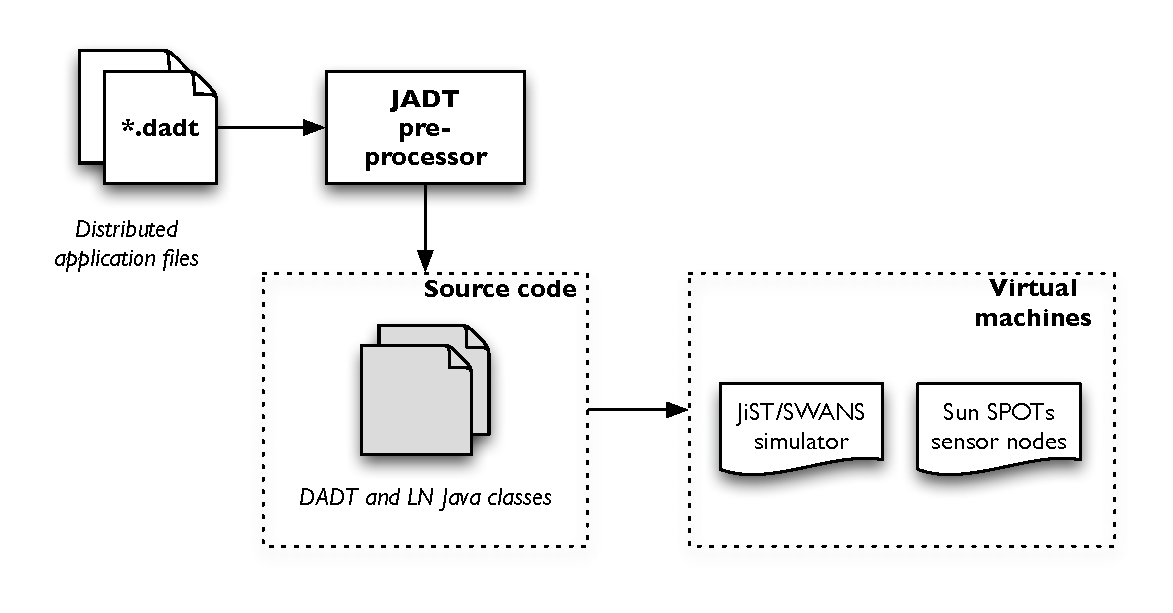
\includegraphics[width=\textwidth]{img/DADTLN_workflow.eps} 
\caption[DADT/LN application workflow]{Workflow for development of an application that uses
the DADT/LN prototype}
\label{Fig:DADTLN_workflow}
\end{figure} 
The overview of the workflow involved in using DADTs to enable WSN application
programming is shown in Figure \ref{Fig:DADTLN_workflow}. The application
developer provides an application layer code for the WSN using a DADT
language in a series of \emph{.dadt} files, that is Java code extended by DADT
constructs. The JADT preprocessor is used to convert the code written by the
application programmer into Java code that interfaces with the DADT infrastructure (extended from the prototype presented in \cite{migliavacca_DADT:2006}). In order to facilitate routing to LNs defined by DADT Views, the DADT infrastructure is interfaced with the a
previously developed implementation of LNs. 

The application (including the implementation of layers lower in the protocol
stack) is then loaded on to either:
\begin{itemize}
\item the JiST/SWANS simulator \cite{barr_JIST:2005, barr_SWANS} (See Section
\ref{sec:jistswans} where implementation details of the simulator are provided) 
\item a collection of Sun SPOT wireless sensor devices
\cite{simon_squawk:2006} (see Section \ref{sec:sunspots}) to execute the given 
application on real sensor nodes.
\end{itemize}

\begin{figure}
\centering
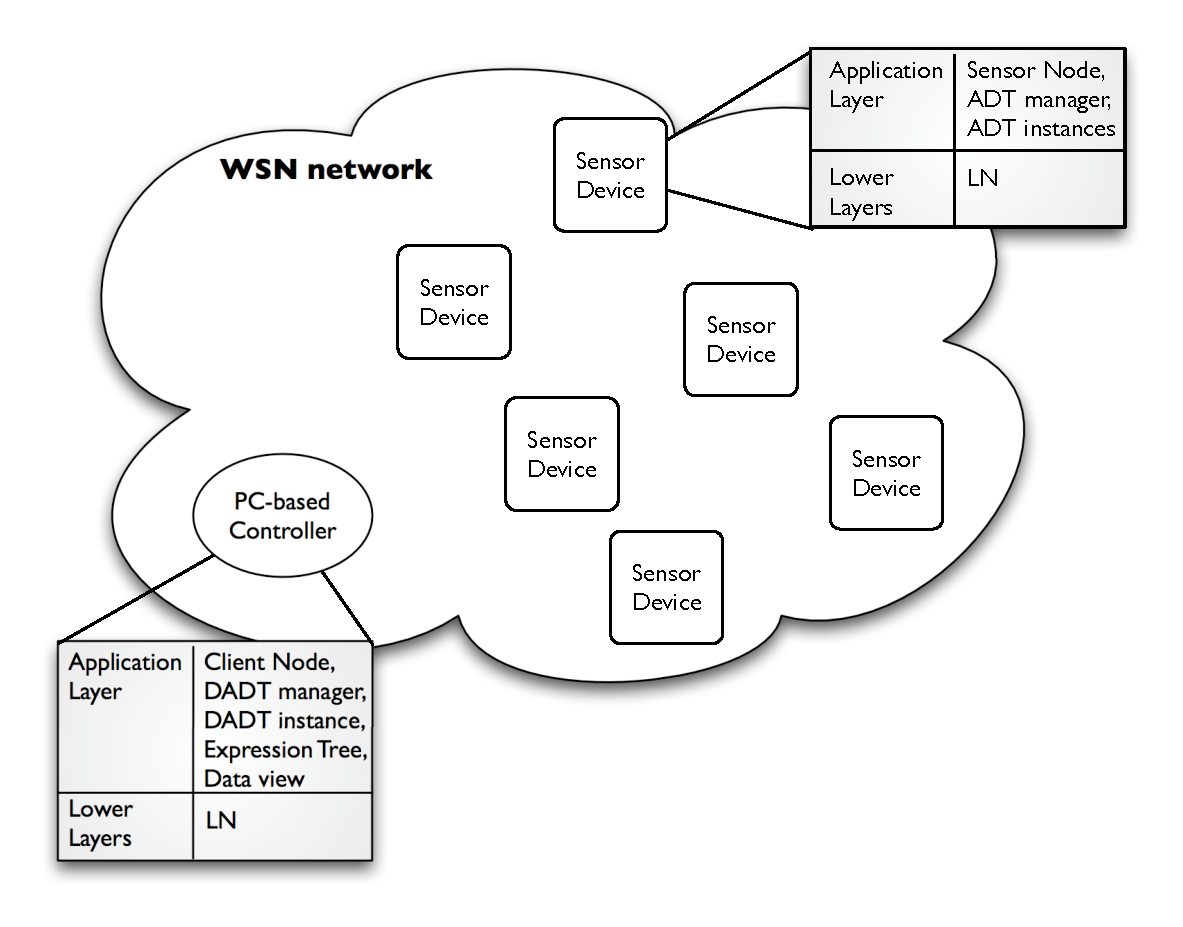
\includegraphics[scale=0.55]{img/DADTLN_glossary.eps} 
\caption[WSN in DADT/LN prototype]{Schematic representation of the WSN as
abstracted in the DADT/LN prototype}
\label{Fig:DADTLN_glossary}
\end{figure} 

The WSN in the DADT/LN prototype developed as part of
this work consists of two types of devices each of which conceal a number
of objects on the different layers of the WSN stack, as shown in Figure
\ref{Fig:DADTLN_glossary}:
\begin{itemize}
  \item \emph{Controller}
  \item \emph{Sensor Device}
\end{itemize}  
   
\emph{Controller} typically resides on a PC. On the application layer, this
abstraction includes the distributed application code, the DADT
instance, and the DADT manager. The Network layer entity hosts the LN implementation.
  
\emph{Sensor Device} is a real-world sensor device such as a Sun SPOT, 
which holds the entities of the application layer, which includes a Sensor Node
abstraction consisting of multiple sensor ADT instances, and an ADT
manager, and a network layer entity which is represented by the LN implementation.

\subsection{Architecture}

The architecture of the DADT/LN prototype is presented in Figure
\ref{Fig:DADTLN_architecture}, and consists of the following logical layers.

\begin{figure}
\centering
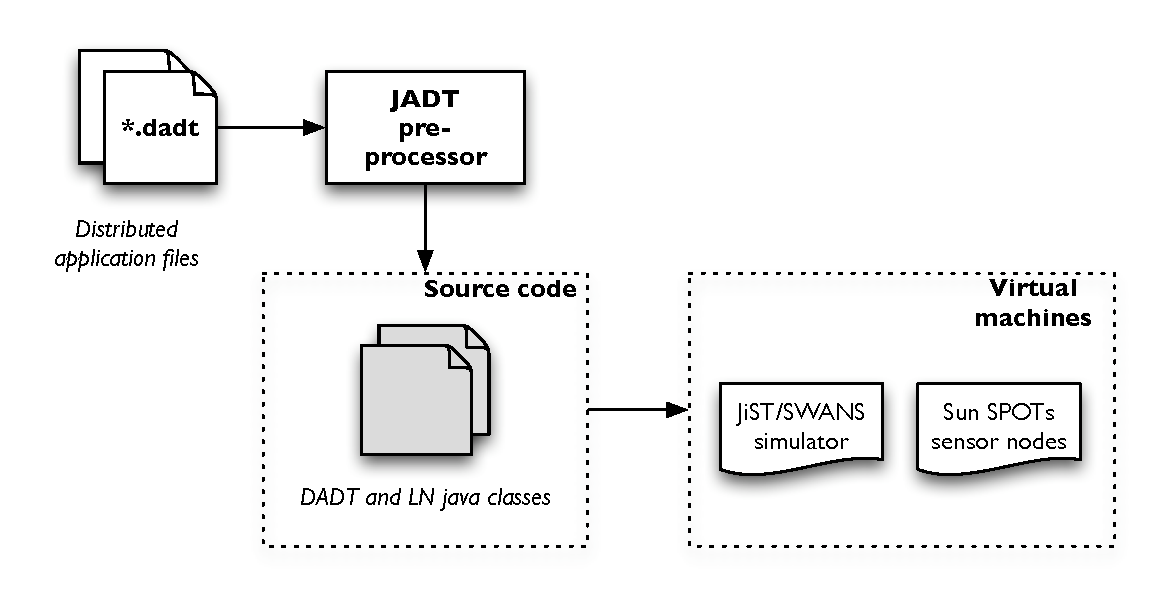
\includegraphics[scale=0.65]{img/DADTLN_architecture.eps} 
\caption[DADT/LN architecture]{Architecture of the DADT/LN prototype}
\label{Fig:DADTLN_architecture}
\end{figure} 

\subsubsection{Upper layer}

The upper layer consists of the following components:

\begin{itemize}
\item \emph {Distributed application}
\item \emph{Sensor} and \emph{DSensor}
\item \emph{DADT runtime layer}
\item \emph{DADT manager}
\item \emph{The Property, Action, and View classes}
\end{itemize}

The Distributed application comprises the code implemented by
the application developer, and is written in Java, extended with constructs defined in the DADT
specification language. This code is later  translated into executable Java
code using a preprocesssor and interfaced with the DADT runtime.

The \emph{Sensor} and \emph{DSensor} classes are the data
ADT and data DADT specifications used by the DADT/LN prototype, and are entirely
defined by the application developer. The space ADTs \emph{Host}
and \emph{Network} are currently built into the DADT/LN prototype, and cannot be defined by the application programmer. However, data ADTs can be placed into space ADTs.

The \emph{DADT runtime layer} holds the DADT runtime library, which provides
handling of ADTs and DADTs. 

The \emph{DADT Manager} performs several tasks, including managing the binding and unbinding
of ADT instances to DADT type by means of the  \emph{Binding Registry} class,
and providing support for space ADTs using the \emph{Site} class. 

The abstract classes \emph{Property} and \emph{Action} represent the
corresponding concepts described in the Section \ref{subsec:DADTsConcepts}.
The class \emph{View} provides support for data and space DADT Views, and
contains the set of \emph{Property} objects that define the scope of the
operations. 

Properties are organised into an abstract tree which provides the
logical predicate defining the view, with the leaves representing DADT
properties and the nodes specifying boolean operators that are used to compose it.
The class \emph{Operator} is a superclass for all of the DADT Operators, though
the current implementation of the DADT/LN prototype provides support mainly for
selection operators.

\subsubsection{Lower Layer}

\emph{DADT/LN runtime} layer provides support for interfacing the DADT runtime
with the LN runtime. This is achived by using instances of the
\emph{LNNodeManager} class on each sensor device and \emph{LNDistrNodeManager}
instance on the controller node.

Communication between sensor devices and the controller node is handled by the LN
runtime layer. This is abstracted from the application programmer by means of the 
\emph{RequestMsg} and \emph{ReplyMsg} methods. The classes \emph{SelectAll} and
o and \emph{SelectAny} implement DADT selection operators, and allow for the invocation of
the corresponding send methods defined in the LN API.

\subsection{Implementation Details}

This section attempts to explain the operation of the DADT/LN prototype
developed as part of this work by considering the sequence of method calls made
during the execution of the DADT/LN prototype. The operation of the simulation platform as well as that of the
nodes themselves are not described in detail in the explanation that follows, as is the actual
\emph{.dadt} syntax used by the application programmer to trigger these
operations. 

\subsubsection{The DADT/LN prototype on the Controller}

Figure \ref{Fig:SeqDiagram_PCnode} presents the operation of the DADT/LN
prototype on the controller. 
Depending on the application purposes the Controller can be run on a separate
node in WSN, or be a PC-based application.

As shown in the figure, the implementation running on the Controller consists of
the following entities:

\begin{itemize}
  \item \emph{Client Node}
  \item \emph{DADT Instance}
  \item \emph{Expression Tree} 
  \item \emph{DADT Manager} 
  \item \emph{Data View} 
\end{itemize}

A \emph{Client Node} is an abstraction that holds a DADT
instance. The application programmer's requests to the network are issued
by the Client Node.
  
A \emph{DADT Instance} allows for collective access to multiple ADT instances (see Section \ref{subsubsec:dadtspecandinst}).

An \emph{Expression Tree} is a special object that allows the construction of an abstract
tree for the DADT View, based on the set of DADT Properties defined.

A \emph{DADT Manager} provides the interface between the Client Node and the
network, and passes request messages from the Client Node to the lower layers
of the protocol stack.

\emph{DADT Views} present a mechanism for partitioning the collection of
ADT instances bound to a particular DADT type, and were explained in Section
\ref{subsubsec:views}.

\begin{sidewaysfigure}[htbp]
\centering
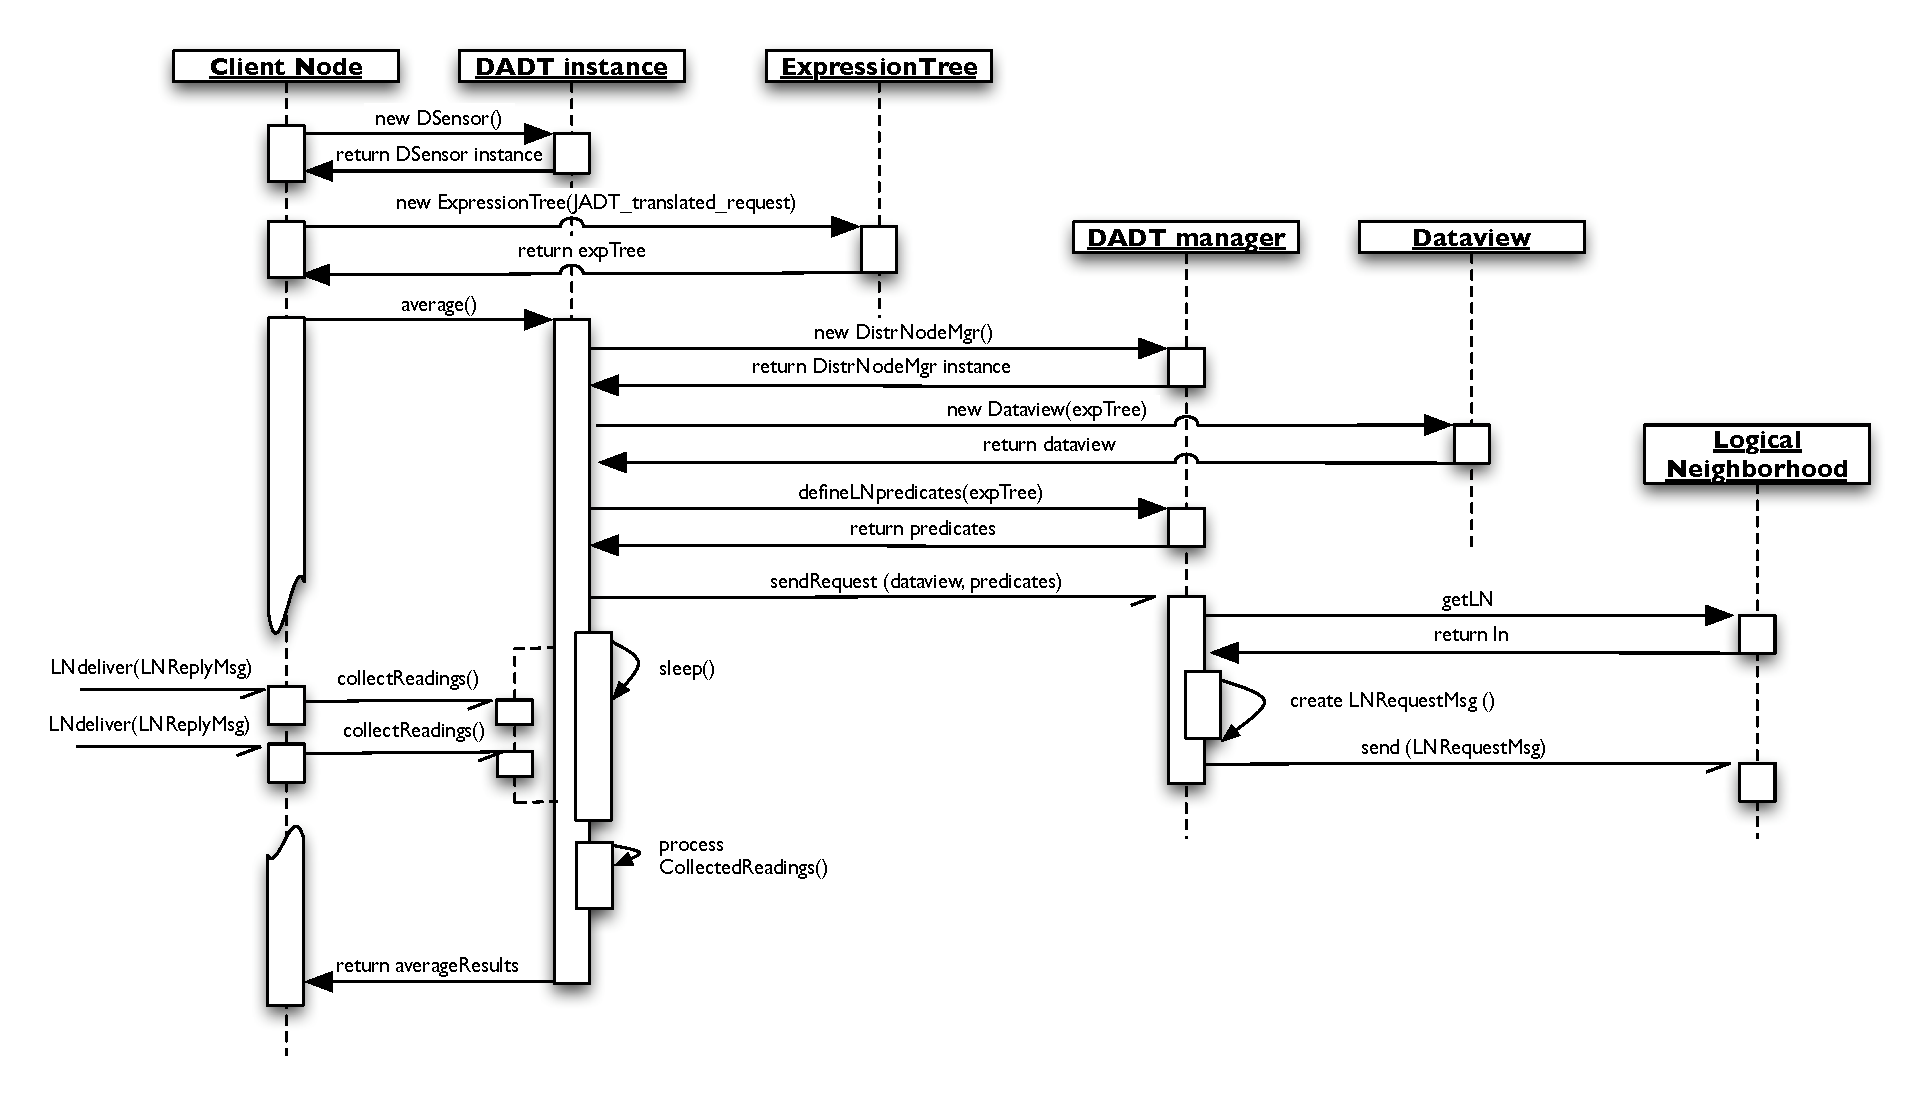
\includegraphics[width=\textwidth]{img/SeqDiagram_PCnode.eps}
\caption[Operation of the DADT/LN prototype on Controller]{Operation of the DADT/LN prototype on Controller}
\label{Fig:SeqDiagram_PCnode}
\end{sidewaysfigure}

The instantiation of a DADT type by the application programmer's
code causes the following actions to take place at the Controller:
\begin{itemize}
 \item the Client Node creates an instance of the DADT type and uses it 
 to perform collective operations on the network.
  \item a new expression tree object 
  is created to provide a representation of the DADT View defined by an application
  programmer.
  \item the DADT instance creates an instance of the DADT Manager.
\end{itemize}

When the application programmer's code requests the execution of a distributed operation
on the WSN, the Client Node forwards the request to the DADT instance, which in turn
processes the request and facilitates communication across the WSN.

The DADT instance performs the following actions:
  \begin{itemize} 
    \item It processes the request, and, according to the defined scope of the
    distributed operation, constructs the relevant DADT View using the
    expression tree object.
    \item It uses the DADT Manager to translate the DADT View
    (defined in the expression tree object) into LN predicates, and constructs and sends a request message to
    underlying WSN.
    \item The DADT instance sleeps until, if required, the result of
    the request is received from the network layer.
  \end{itemize}
  
If no reply is expected from the nodes to which the communication was sent, the Client Node continues to operate normally. This situation occurs, for instance, in the case of a request from the Controller Node
that contains the \emph{ResetAll} action. 
 
Otherwise, if the result of the distributed computation is expected, the DADT
instance is notified when the relevant data are received from the WSN.
The DADT instance then invokes the relevant methods to collect and process the received
readings. Finally, it returns the result of the DADT request to
the Client Node.

\subsubsection{The DADT/LN prototype on the sensor device} \label{subsubsec:DADTLNSensorDevice}

Figure \ref{Fig:SeqDiagram_Sensornode} presents the operation of the DADT/LN
prototype on the sensor device (which may be either a simulated or a real
node).

In the rest of this section, the term \emph{sensor device} is used to refer to the
physical sensor node entity, while the term \emph{sensor node} refers to the application
layer abstraction of all of the sensors within the device that resides on-device.

The DADT/LN prototype implementation running on each sensor node consists of the
following entities:

\begin{itemize}
  \item \emph{Sensor Node} 
  \item \emph{Sensor ADT instance} 
  \item \emph{ADT Manager} 
\end{itemize}

A \emph{Sensor Node} is an abstraction that consists of a list of sensors. This
follows from the example used to illustrate the concept of ADTs in Section
\ref{subsec:ADTSpecInst}. 

A \emph{Sensor ADT instance} is an ADT instance for a given sensor on the sensor
node upon which the prototype executes.

An \emph{ADT Manager} provides the interface between the sensor node and the
network, thereby abstracting sensor ADT instances from queries issued by the DADT
instance at the (PC-based) controller.

\begin{sidewaysfigure}[htbp]
\centering
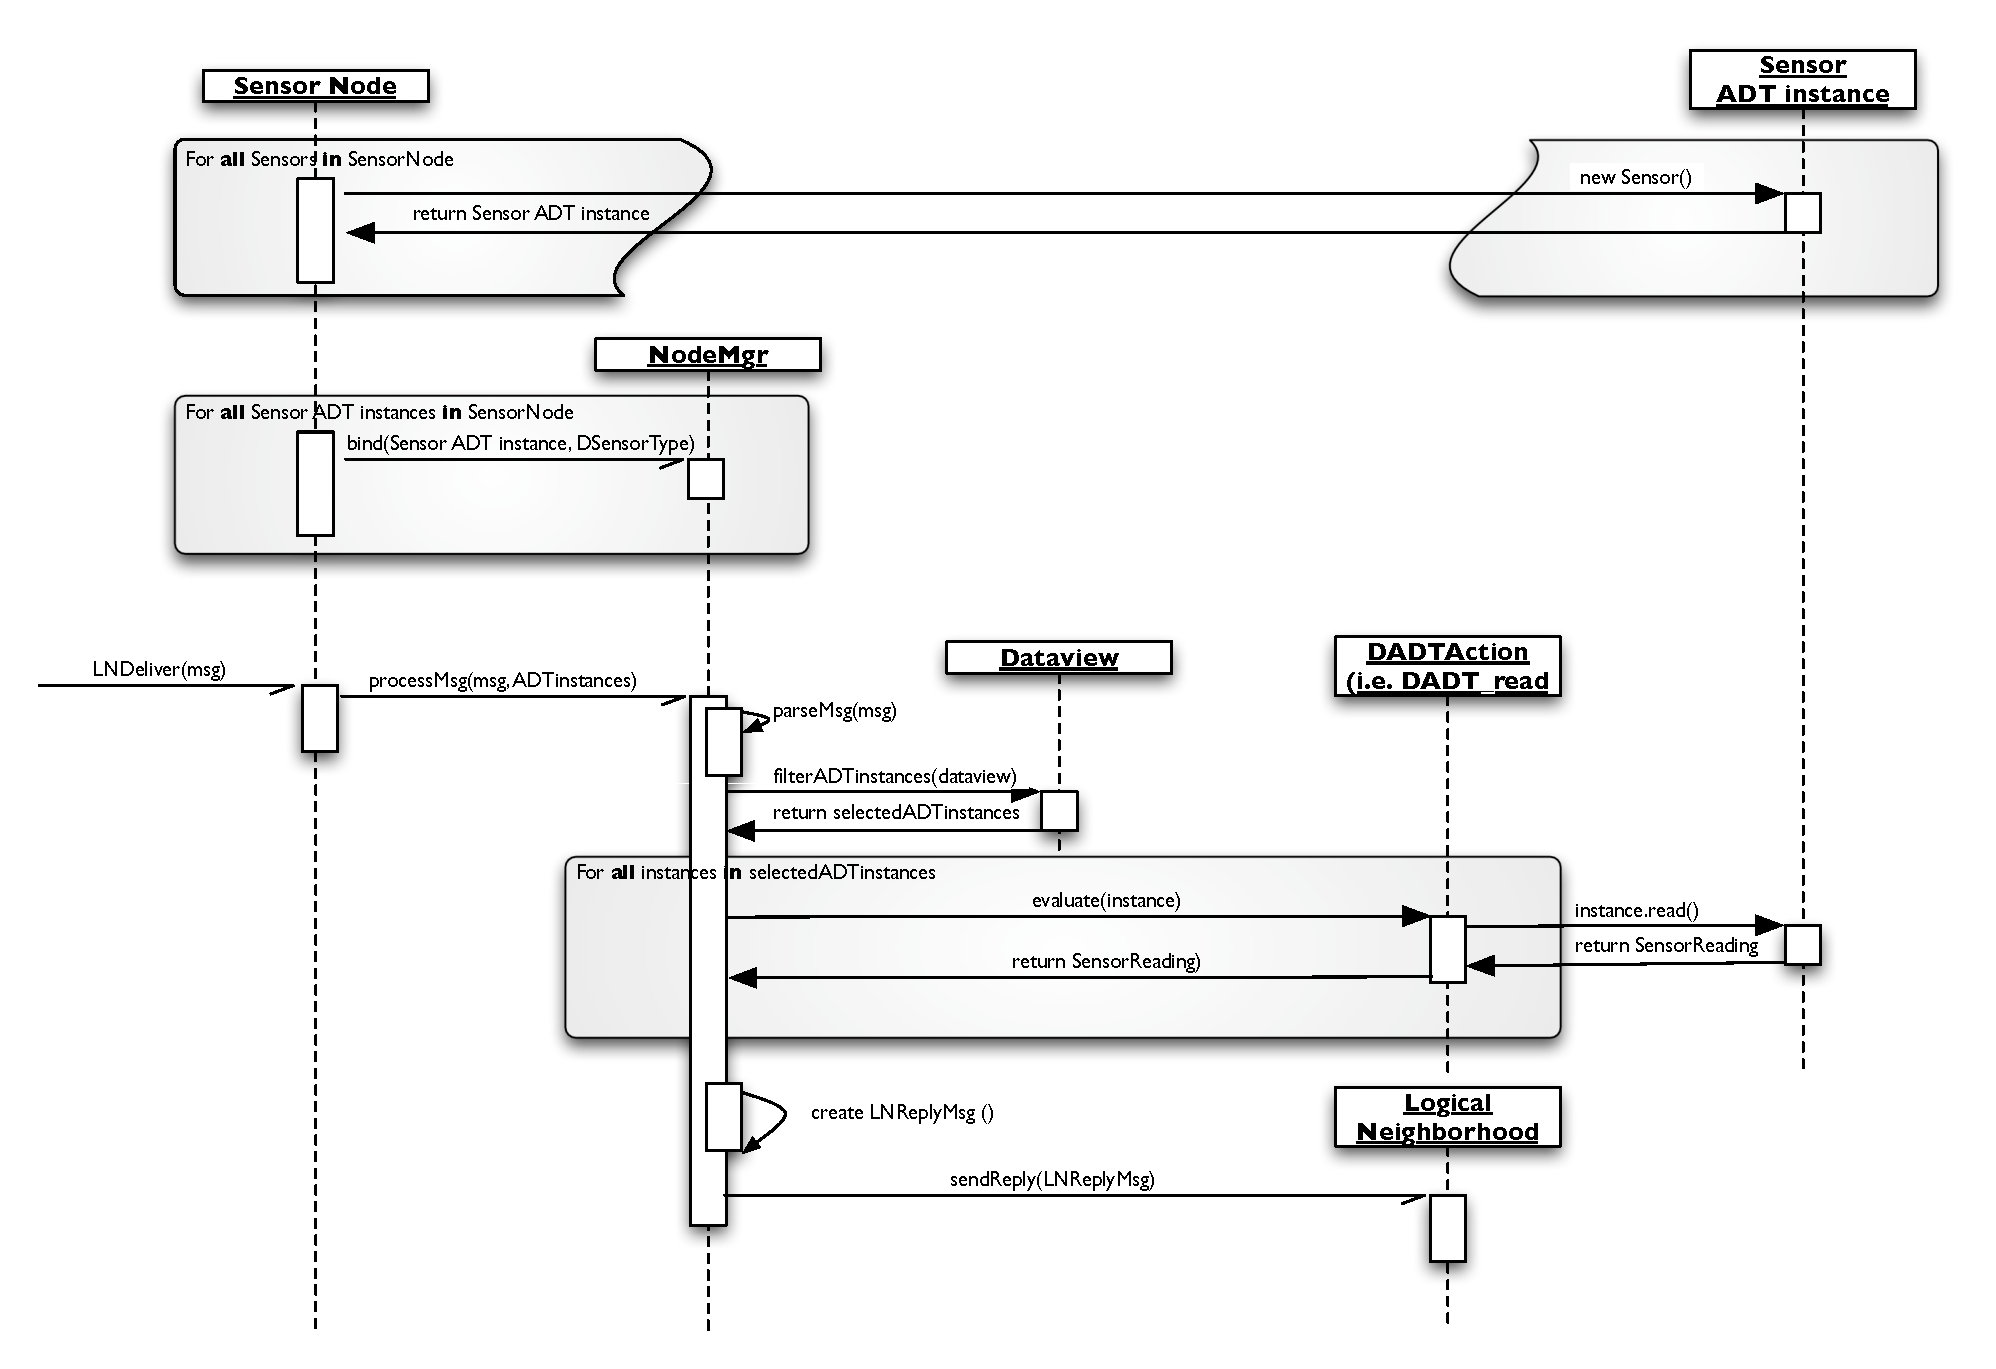
\includegraphics[width=\textwidth]{img/SeqDiagram_Sensornode.eps}
\caption[Operation of the DADT/LN prototype on sensor device]{Operation of the DADT/LN prototype on sensor device}
\label{Fig:SeqDiagram_Sensornode}
\end{sidewaysfigure}

Intialisation of the Sensor ADT instance is performed possibly
multiple times on a given Sensor Node, as a node might consist of multiple sesnsors. Following
this, the sensor ADT instances are bound to a particular DADT type by calling
the ADT manager\footnote{The ADT manager is assumed in our
current implementation to be aware of all DADT types defined in the WSN.}.

When the lower layer (which runs the LN algorithm) delivers a message to the
Sensor Node, the ADT Manager is used to process the request message.The
request message contains details of the DADT View (see Section
\ref{subsubsec:views}) used later to filter from the sensor ADT
instances on the given Sensor node those that fit into the requested DADT View. 

If the request message is received in the application layer, then at least one of
the sensor ADT instances in the Sensor Node fits into the DADT view, as the DADT
view is expressed in the form of LN predicates\footnote{If none of the sensor ADT instances fit the view, the message would be discarded in the network layer.}. This minimises the number of
messages received at the application layer. However, since a given Sensor Node
may contain several sensor ADT instances, the ADT instances have to be filtered.

The request message also contains information about the DADT action to be
performed on device (see Section \ref{subsubsec:OperatorsAndActions}). 
The ADT manager calls the action for each sensor ADT instance that fits into the DADT View. 

If the application layer requires that a reply be sent, the LN implementation in
the lower layer of the protocol stack is used as can be seen on the bottom
right section of Figure \ref{Fig:SeqDiagram_Sensornode}.


\subsection{The DADT/LN prototype in the simulated environment}
\subsubsection {JiST/SWANS} \label{sec:jistswans}

As the simulator used in this work is a discrete event simulator, this section 
begins with a short description of discrete event simulators. 
This is followed by a discussion on the SWANS network simulator used during the course of this work, and the JiST Java-based discrete event simulator upon which SWANS is built.

\paragraph{Discrete Event Simulator}

A discrete event simulator allows for the simulated execution of a process (that
may be either deterministic or stochastic), and consists of the following
components \cite{Shankar_DiscreteEventSim}:

\begin{itemize}
  \item \emph{Simulation variables:} These variables keep track of simulation 
  time, the list of events to be simulated, the (evolving) system state, and 
  performance indicators.
  \item \emph{Event handler:} The event handler schedules events for execution 
  at specific points in simulation time (and unschedules them if necessary), 
  and additionally updates the state variables and performance indicators.
\end{itemize}
 
\paragraph{Java In Simulation Time (JiST)} \label{subsec:jist}

JiST \cite{barr_JIST:2005} is a discrete event simulator that is 
efficient (compared to existing simulation systems), 
transparent (simulations are automatically translated to run with the 
simulation time semantics), and standard (simulations use a
conventional programming language, i.e., Java).

JiST simulation code is written in Java, and converted to run over the JiST 
simulation kernel using a bytecode-level rewriter\footnote{The bytecode 
rewriter and the simulation kernel are both written in Java},  as can be
seen in Figure \ref{Fig:JiST_architecture}.

The execution of a JiST program can be understood by considering the example 
shown in Listing \ref{listing:JiSTExample}

\begin{lstlisting}[frame=trbl, basewidth={0.55em, 0.6em}, captionpos=b, 
basicstyle=\ttfamily\footnotesize, breaklines, caption = Example JiST program (reproduced from \cite{barr_JIST:2005}, label = listing:JiSTExample]  
import jist.runtime.JistAPI;  
class hello implements JistAPI.Entity { 
  public static void main(String[] args) { 
    System.out.println("Simulation start"); 
    hello h = new hello(); 
    h.myEvent(); 
  } 
  public void myEvent() { 
    JistAPI.sleep(1); 
    myEvent(); 
    System.out.println("hello world, " + JistAPI.getTime()); 
  }} 
\end{lstlisting}

\begin{figure}
\centering
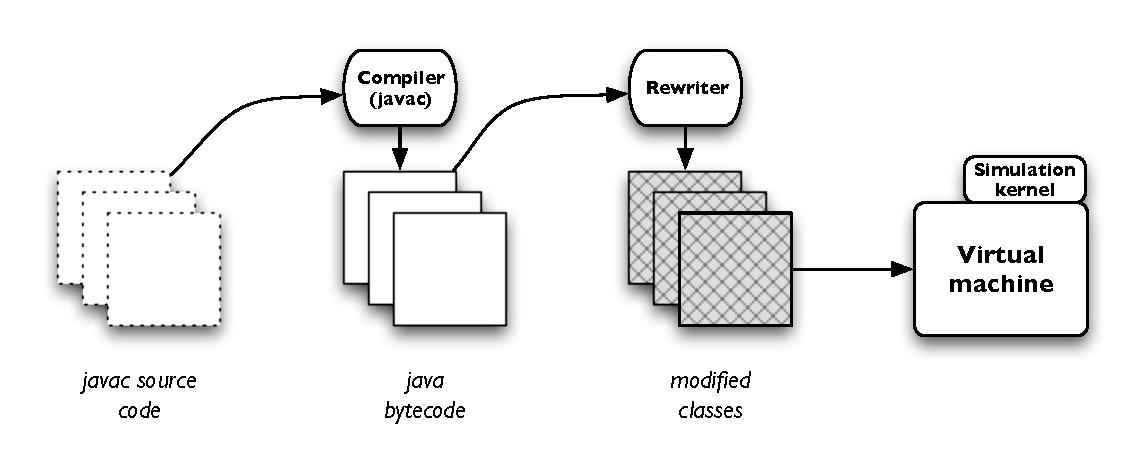
\includegraphics[width=\textwidth]{img/JiST_architecture.eps} 
\caption[The JiST System Architecture]{The JiST system architecture (reproduced from
\cite{barr_JIST:2005})}
\label{Fig:JiST_architecture}
\end{figure}  
 
This program is then compiled and executed in the JiST simulation
kernel, using the following commands:

  
\begin{lstlisting}[frame=trbl, basewidth={0.55em, 0.6em}, captionpos=b, 
basicstyle=\ttfamily\footnotesize, breaklines, caption = Execution of the
program in the JiST, label = listing:JiST ]  
javac hello.java
java jist.runtime.Main hello
\end{lstlisting}


The simulation kernel is loaded upon execution of this command. This kernel
installs into the JVM a class loader that performs the rewrite of the bytecode.
The JistAPI functions used in the example code are used to perform the
code transformations. The method call to myEvent is now scheduled and executed
by the simulator in simulation time. Simulation time differs from ``actual''
time in that the advancement of actual time is independent of application
execution, whereas simulation time is not. 
 
\paragraph{Scalable Wireless Ad hoc Network Simulator (SWANS)}
SWANS is a wireless network simulator developed in order to provide efficient
and scalable simulations without compromising on simulation detail \cite{barr_SWANS},
and is built upon the JiST discrete event simulator described in Section \ref{subsec:jist}. 
It is organised a a collection of independent, relatively simple, event driven
components that are encapsulated as JiST entities. 

\begin{figure}[h]
\centering
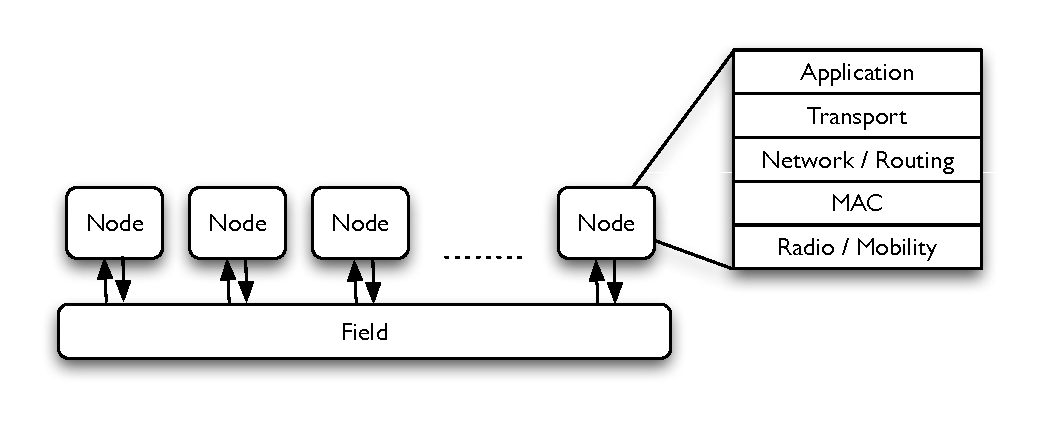
\includegraphics[width=\textwidth]{img/SWANS_architecture.eps} 
\caption[SWANS architecture]{SWANS architecture}
\label{Fig:SWANS_architecture}
\end{figure} 
  
SWANS has the following capabilities \cite{barr_SWANS}:

\begin{itemize}
\item The use of
interchangeable components enables the construction of a protocol stack for the
network, and facilitates parallelism, and execution in a distributed environment.
\item Can execute unmodified Java network applications on the
simulated network (in simulation time), by virtue of its being built over
JiST.Using a harness, the aforementioned Java code is automatically rewritten to
run on the simulated network.  
\end{itemize}
   
The SWANS architecture may be seen in Figure \ref{Fig:SWANS_architecture}. 


\subsubsection{Simulation using JiST/SWANS}

The DADT/LN prototype was tested on the SWANS WSN simulator, which is built upon
the JiST discrete event simulator (see Section \ref{subsec:jist}). 

The DADT/LN prototype code is wrapped in the JiST API, and is loaded on to a
simulated node. As described in the previous section, there are two kinds of
nodes in the DADT/LN prototype:

\begin{itemize}
  \item \emph{Controller Node}, which holds the distributed application, and the
  framework to manage the same.
  \item \emph{Sensor Device}, which holds the individual ADT instances. 
\end{itemize}

The Controller Node was implemented as a separate node on the JiST/SWANS
simulator, and was run as an independent simulated node for the purposes of
the simulation. The Sensor Device implementation (see Section
\ref{subsubsec:DADTLNSensorDevice}) was loaded on to all but one of the nodes in
the simulator.

The simulation was run on networks of upto 50 nodes to develop and empirically verify the
robustness of the work done as part of this thesis.

\subsection{The DADT/LN prototype on Sun SPOTs}

For further experimental validation of the implementation produced as part of 
this thesis, the DADT/LN prototype was deployed on Sun SPOTs \cite{simon_squawk:2006} (see Section \ref{sec:sunspots}. 

The Controller application was executed as a host application on the host machine (a
PC), while the other Sun SPOTs ran the Sensor Device implementation as on-SPOT
applications (see Section \ref{subsec:sunspotapps} for a description of host and on-SPOT
applications).

Deployment of the DADT/LN prototype on Sun SPOT devices involved several
challenges. Whereas the JiST/SWANS simulator allows to run unmodified Java code on
the simulated node, the Squawk JVM on Sun SPOTs introduces severe limitations
on the code. The application code has to be compliant with CLDC 1.1
specification of Java ME, and therefore lacks support for a number of APIs that were previously used during the development of the DADT prototype \cite{migliavacca_DADT:2006}.